% Long: they only share an instruction when it is the same. They do not do
% anything to synchronize the threads.

% 

\documentclass[times,10pt,twocolumn]{article} 

\usepackage{tikz}
\usepackage{caption}
\usepackage{amsfonts}
\usepackage{enumitem}
\usepackage{subcaption}
%\usepackage[lined,ruled,linesnumbered]{algorithm2e}

\usepackage{amsmath,amssymb}
\usepackage{fullpage}
\usepackage{graphicx}
\usepackage{setspace}
\usepackage{stmaryrd}
%\usepackage{proof}
\usepackage{skak} % for the \qside
\usepackage{array}
\usepackage{url}

\usetikzlibrary{positioning,shapes.geometric}
\usetikzlibrary{arrows}
\usetikzlibrary{automata}

\newtheorem{theorem}{Theorem}[section]
\newtheorem{corollary}[theorem]{Corollary}
\newtheorem{definition}[theorem]{Definition}

\newcommand{\tid}{\mbox{\texttt{T}}_{id}}
\newcommand{\simd}{$\mu$-\textsc{Simd}}
\newcommand{\code}[1]{\mbox{\texttt{#1}}}

\begin{document}

\title{Fusion of calling sites
\thanks{This work was partially supported by CNPq, CAPES, FAPEMIG.}
}

\author{Douglas do Couto Teixeira ~~ Sylvain Collange ~~ Fernando Magno Quint\~{a}o Pereira\\
Departamento de Ci\^{e}ncia da Computa\c{c}\~{a}o ~~
Universidade Federal de Minas Gerais, Brazil\\
{\small {\tt \{douglas,sylvain.collange,fernando\}@dcc.ufmg.br}}
} 

\maketitle
\thispagestyle{empty}

\maketitle

\begin{abstract}
% Context
The increasing popularity of Graphics Processing Units (GPUs), has brought
renewed attention to old problems related to the Single Instruction, Multiple
Data execution model.
% Problem
One of these problems is the reconvergence of divergent threads.
A divergence happens at a conditional branch when different threads disagree on
the path to follow upon reaching this split point.
Divergences may impose a heavy burden on the performance of parallel programs.
% Solution
In this paper we propose a compiler-level optimization to mitigate this
performance loss.
This optimization consists in merging function call sites located at different
paths that sprout from the same branch.
% Results
We show that our optimization adds negligible overhead on the compiler.
It does not slowdown programs in which it is not applicable, and accelerates
substantially those in which it is.
As an example, we have been able to speed up the well known SPLASH Fast Fourier
Transform benchmark by 11\%.
\end{abstract}

%%%%%%%%%%%%%%%%%%%%%%%%%%%%%%%%%%%%%%%%%%%%%%%%%%%%%%%%%%%%%%%%%%%%%%%%%%%%%%%%

\section{Introduction}
\label{sec:int}

% Context:
Graphics Processing Units (GPUs) are becoming a staple hardware in the
high-performance world.
They provide a simple, cheap, and efficient platform in which parallel
applications can be developed~\cite{Nickolls10}.
Since the release of CUDA, in early 2006~\cite{Garland08}, a plethora
of programming patterns and algorithms have been designed to run in this
environment, touching multiple fields of knowledge, including Biology,
Chemistry and Physics~\cite{Navarro14}.

The basic operating principle of this
hardware consists in running the threads of {\em Single Program, Multiple
Data} (SPMD) programs in lockstep, so to execute their identical instructions on
{\em Single Instruction, Multiple Data} (SIMD) units.
This execution model is, nowadays, known as {\em Single Instruction, Multiple
Threads} (SIMT), a term coined by Nvidia's engineers~\cite{Nickolls10}.
SIMT execution has gained momentum beyond the graphics processing ecosystem.
SPMD programming environments like OpenCL\footnote{\url{http://www.khronos.org/opencl/}}, 
OpenACC\footnote{\url{http://www.openacc.org/}} or
OpenMP 4.0\footnote{\url{http://openmp.org/}} can target SIMD architectures like
GPUs, multi-core CPUs with SIMD extensions, and even Intel Xeon Phi accelerators.

% Problem:
Nevertheless, in spite of all these advances, programming SPMD applications for
SIMD architectures remains a challenging task.
One of the reasons behind this difficulty is a phenomenon known as
{\em Thread Divergence}.
When facing a conditional branch, two threads diverge if 
they disagree on which path to take.
Divergences are a problem because they have an impact on the program's
performance.
In other words, a divergence splits threads into two groups, upon reaching a
conditional branch.
Only one of these groups contain threads that do useful work at a given point
in time.

% Solution:
We have designed, implemented and tested a compiler optimization that
mitigates this performance loss.
We name this optimization {\em Fusion of Calling Sites} (FCS).
Our optimization relies on a simple idea: threads should enter functions
in lockstep to minimize the effects of divergences.
Therefore, whenever a function is invoked at the two different paths that stem
from a conditional test, we merge the two calling sites into one single
invocation of that function.
This optimization can benefit implicit SIMD architectures, such as those found in
GPUs, and explicit SIMD hardware like the Xeon Phi.
In the latter case, the compiler merges threads together to form SIMD instruction,
handling divergence with mask-predicated instructions~\cite{Karrenberg12}.

% Result:
As we show in Section~\ref{sec:sol}, our algorithm scans blocks of code within
the program, performing the merging whenever it is possible.
In this paper, we demonstrate that our optimization is:
(i) easy to implement, (ii) innocuous when non-applicable and
(iii) effective when used.
Our optimization has low computational complexity in practice.
In other words, it always applies a constant number of
operations per pair of calling sites that it merges.
If a program does not present any opportunity for this merging to happen,
then we do not impose any runtime overhead onto the compiler, nor onto the
executable program, once it is deployed.
In Section~\ref{sec:exp}, we show the potential of our optimization through a
toy benchmark, and show its applicability in the well-known implementation of
Fast Fourier Transform available in SPLASH\footnote{\url{http://www.capsl.udel.edu/splash/}}.
In the former benchmark, FCS reduces the number of divergent instructions by
55\%, and on the latter by 11\%.

\section{Overview of the Approach}
\label{sec:ovf}

\begin{figure}[b!]
\begin{center}

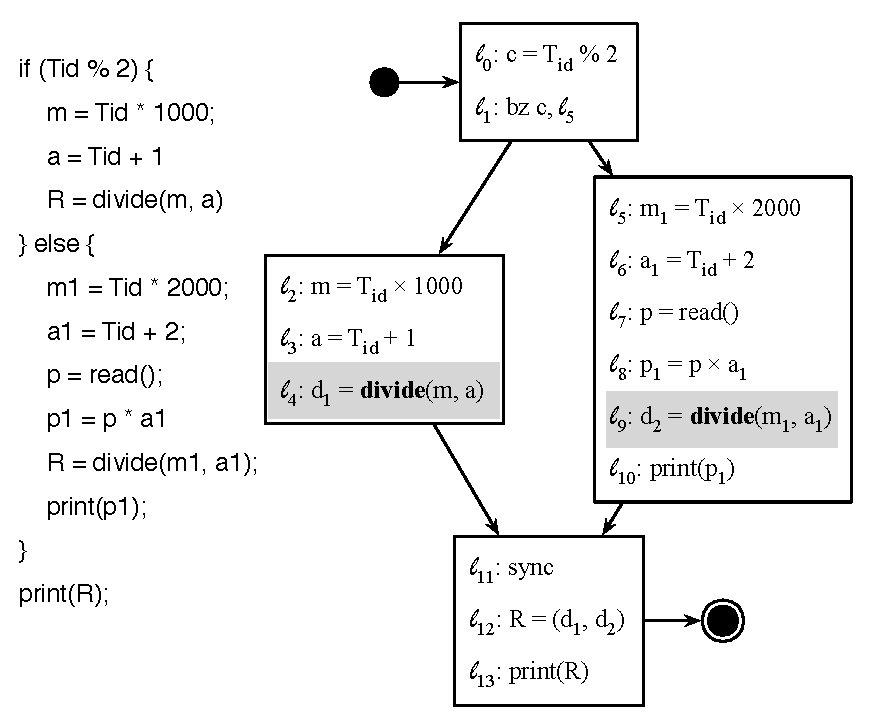
\includegraphics[width=1\columnwidth]{images/divide0} \\
\begin{small}
\begin{tabular}{|c|l|c|c|c|c|} \hline
Cycle   & Instruction                  & $t_0$        & $t_1$        & $t_2$        & $t_3$        \\ \hline
14      & $ c = \tid \% 2$             & $\checkmark$ & $\checkmark$ & $\checkmark$ & $\checkmark$ \\ \hline
15      & $ \code{bz} \ c, then$ & $\checkmark$ & $\checkmark$ & $\checkmark$ & $\checkmark$ \\ \hline
16      & $ m = \tid \ \times \ 1000$        & $\checkmark$    & $\bullet$ & $\checkmark$ & $\bullet$ \\ \hline
17      & $ a = \tid \ + \ 1$ & $\checkmark$    & $\bullet$ & $\checkmark$ & $\bullet$ \\ \hline
18      & $ d1 = divide(m, a)$ & $\checkmark$    & $\bullet$ & $\checkmark$ & $\bullet$ \\ \hline
\multicolumn{6}{c}{$\ldots$} \\ \hline
118      & $ m1 = \tid \ \times 2000$ & $\bullet$    & $\checkmark$ & $\bullet$ & $\checkmark$ \\ \hline
119     & $ a1 = \tid \ + \ 2$        & $\bullet$    & $\checkmark$    & $\bullet$ & $\checkmark$ \\ \hline
120     & $ p = read()$ & $\bullet$    & $\checkmark$    & $\bullet$ & $\checkmark$ \\ \hline
121     & $ p1 = p \ \times a1$ & $\bullet$    & $\checkmark$ & $\bullet$ & $\checkmark$ \\ \hline
122     & $ d2 = divide(m, a)$        & $\bullet$    & $\checkmark$    & $\bullet$ & $\checkmark$ \\ \hline
\multicolumn{6}{c}{$\ldots$} \\ \hline
222      & $ print(p1)$ & $\bullet$    & $\checkmark$    & $\bullet$ & $\checkmark$ \\ \hline
223     & $ \code{sync}$        & $\checkmark$ & $\checkmark$ & $\checkmark$ & $\checkmark$ \\ \hline
224     & $ R = phi(d1, d2)$    & $\checkmark$ & $\checkmark$ & $\checkmark$ & $\checkmark$ \\ \hline
225     & $ print(R)$ & $\checkmark$    & $\checkmark$ & $\checkmark$ & $\checkmark$ \\ \hline
\end{tabular}

\end{small}
\end{center}
\caption{(Top) A program whose performance may experience a
slowdown due to divergences.
(Bottom) An execution trace of the program.
If a thread $t$ executes an instruction at cycle
$j$, we mark the entry $(t, j)$ with $\checkmark$.
Otherwise, we mark it with $\bullet$.
In this example we assume that each invocation of function \texttt{divide} takes
one hundred cycles to execute.}
\label{fig:exampleOrig}
\end{figure}

Figure~\ref{fig:exampleOrig} will let us illustrate thread divergences.
This phenomenon characterizes the Single Instruction, Multiple Data
execution model typical of Graphics Processing Units.
These processors organize threads in groups that execute in lockstep.
Such groups are called {\em warps} in NVIDIA's jargon, or {\em wavefronts} in
AMD's.
We can imagine that threads in the same warp use different arithmetic and
logic units, but share the same instruction control logic.
Control flow divergences happen when threads
in a warp follow different paths after processing the same branch.
If the branching condition is data divergent, then it might be true to some
threads, and false to others.
In face of divergences, some threads will take the ``then" part of the branch
in Figure~\ref{fig:exampleOrig}, and others will take the ``else" part.
Due to the shared instruction control logic, only one group
of threads will be allowed to do useful work at a given instant.
The execution trace at the bottom of Figure~\ref{fig:exampleOrig} shows
which threads are active at each cycle, assuming an architecture that allows
four threads simultaneously in flight.

When two threads diverge, the hardware should reconverge them as earlier as
possible to maximize the amount of active workers per cycles.
A {\em reconvergence point} is the earliest instruction in the program where we
can expect control flow paths to join regardless of the outcome or target of
the divergent branch.
Fung {\em et al.} have shown that the {\em post-dominator} of a branch is --
usually -- the best place to reconverge threads~\cite{Fung07}.
We say that a node $v$ in a CFG post-dominates a node $u$ if any path from $v$
to the end of the CFG must go across $u$.
In Figure~\ref{fig:exampleOrig}, basic block \texttt{end} is the post-dominator
of every other block.
Yet, as Fung {\em et al.} themselves have also shown, reconverging threads at the
post-dominators of branches is far from being a perfect solution to divergences.
Figure~\ref{fig:exampleOrig} illustrates this situation particularly well.

The \texttt{divide} function is invoked at both sides of the branch in
Figure~\ref{fig:exampleOrig}.
Even though this function must be executed by all the threads that reach the
divergent branch, these threads will be entering the function at different
execution cycles due to the divergence.
Consequently, the instructions that constitute function \texttt{divide} will
be called twice: once for the threads in the ``then" part of the branch, and
another time for the threads in the ``else" part.
In this case, reconverging threads at post-dominators of divergent points will
not avoid the redundant execution of \texttt{divide}.
If \texttt{divide} runs for a long time, then we will be missing the
opportunity to share many execution cycles among different threads.
The goal of FCS is to reconverge threads at the entry points
of functions.
We will accomplish this goal by changing the structure of the program's
control flow graph, as we will explain in the next section.

\section{Fusion of Calling Sites}
\label{sec:sol}

% High level description
Figure~\ref{fig:Algorithm0} provides a high-level view of FCS.
The function \textbf{merge\_call\_site} tries to join call sites, until this
action is no longer possible.
If a merging happens, then the function invokes itself recursively, otherwise
the optimization terminates.
Candidate branches are found via the function \textbf{find\_joinable\_calls},
which is also depicted in Figure~\ref{fig:Algorithm0}.
This procedure looks for paths that stem from the same branch $\ell_b$ and that
lead to different calls of the same function $F$.
If the {\em cost} of transforming the program's control flow graph is lower than
a certain {\em threshold}, then the prospective branch is sent to function
\textbf{merge\_cfg}, which is in charge of transforming the program.

\begin{figure}[hbt]
\begin{center}
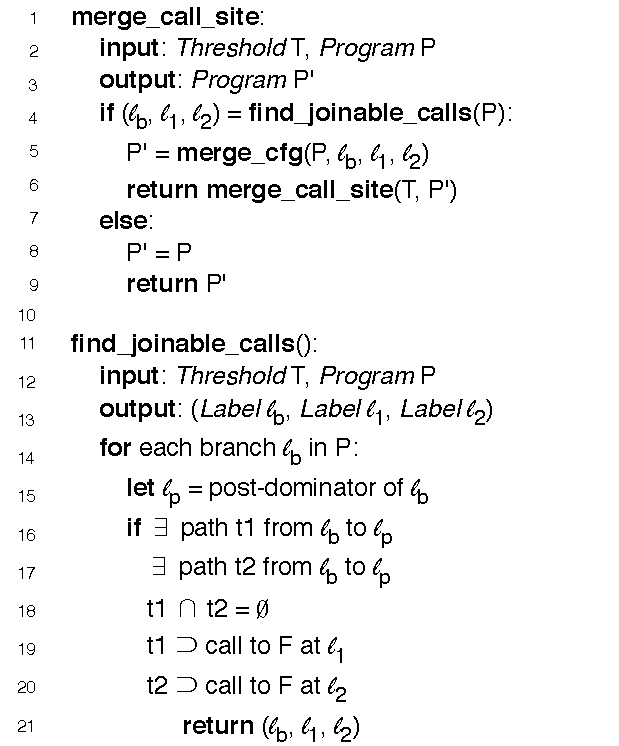
\includegraphics[width=1\columnwidth]{images/Algorithm0}
\end{center}
\caption{\label{fig:Algorithm0}
Main routines that perform the fusion of calling sites.}
\end{figure}

\begin{figure}[hbt]
\begin{center}
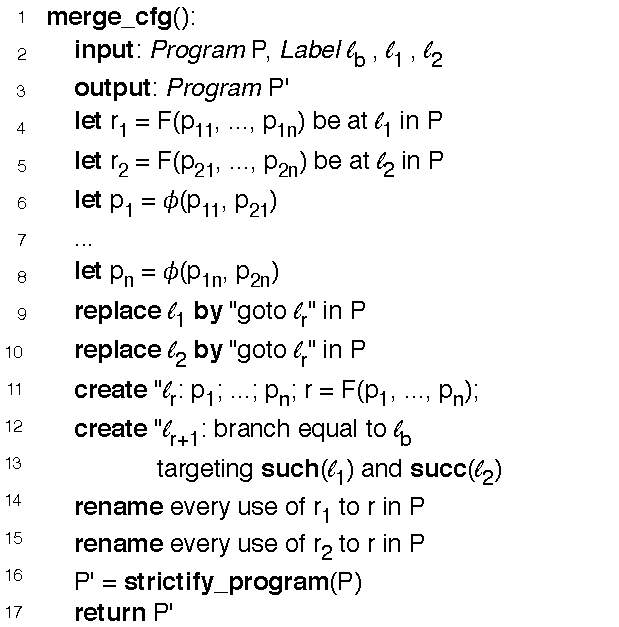
\includegraphics[width=1\columnwidth]{images/merge_cfg}
\end{center}
\caption{\label{fig:merge_cfg}
Routine that transforms the program's control flow graph.
We let succ($\ell$) be the unique successor of label $\ell$.}
\end{figure}

% Example
We use the program from Figure~\ref{fig:exampleOrig} as an example to
illustrate our transformation.
The program in that figure has one candidate branch, at label $\ell_1$.
Our function \textbf{find\_joinable\_calls} will detect two paths from this
branch leading to invocations of the same function.
The first path is formed by the sequence of labels $\ell_1 \rightarrow \ell_2
 \rightarrow \ell_3 \rightarrow \ell_4$.
The second path if formed by the sequence $\ell_1 \rightarrow \ell_5
 \rightarrow \ell_6 \rightarrow \ell_7 \rightarrow \ell_8 \rightarrow \ell_9$.
After finding the paths, our routine \textbf{merge\_cfg} will produce a new
version of the program.

Figure~\ref{fig:OverviewTransform} provides an overview of the
transformation that \textbf{merge\_cfg} performs.
This function creates a common label, e.g., $\ell_r$, that will join the
two call sites that we want to fuse.
We use the $\phi$-functions of the {\em Static Single
Assignment}~\cite{Cytron91} (SSA) form to join function arguments.
SSA form is a program representation in which each variable has only one
definition site~\cite{Cytron91}.
Nowadays, almost every compiler uses this intermediate representation to
manipulate programs.
The SSA format relies on $\phi$-functions to join different variables into
common names.
Going back to Figure~\ref{fig:OverviewTransform}, an instruction such as
$a_1 =\phi(a_{11}, a_{21})$ will assign to variable $a_1$
the value of $a_{11}$ if the program flow reaches that operation through label
$\ell_1$, and will assign $a_{21}$ to $a_1$, if the program flow comes through
label $\ell_2$.
Figure~\ref{fig:Algorithm1} shows the program that we obtain after applying
the FCS optimization onto the function seen in Figure~\ref{fig:exampleOrig}.
This time we have only one invocation site for function \textbf{divide}, which
will be reached independent on the way that we branch at $\ell_1$.
The branch immediately after the new label $\ell_r$ is used to preserve the
program flow after the execution of \textbf{divide}.

\begin{figure}[t!]
\begin{center}
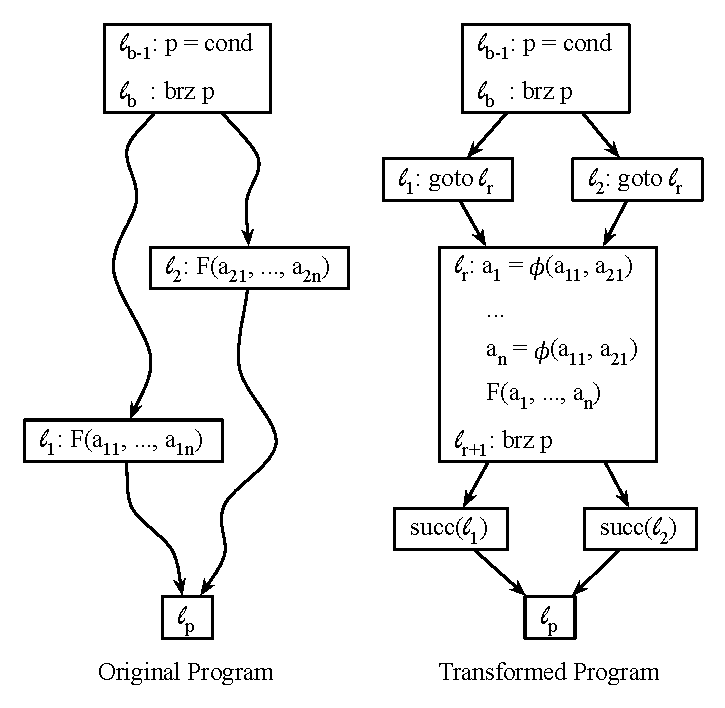
\includegraphics[width=1\columnwidth]{images/OverviewTransform}
\end{center}
\caption{\label{fig:OverviewTransform}
Overview of the transformation that we perform to join function calls.}
\end{figure}


\begin{figure}[hbt]
\begin{center}
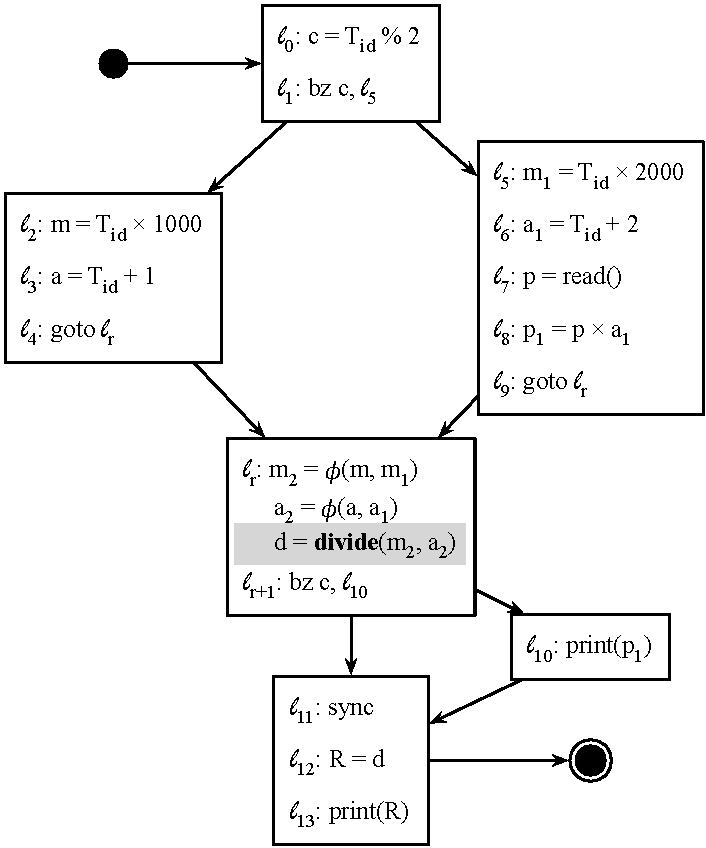
\includegraphics[width=1\columnwidth]{images/Algorithm1}
\end{center}
\caption{\label{fig:Algorithm1}
Transformed version of the program earlier seen in Figure~\ref{fig:exampleOrig}.}
\end{figure}

% Strictification
\noindent
\textbf{Ensuring Strictness: }
We notice that the transformed program contains a path in which variable $p_1$
is used without being defined: $\ell_0 \rightarrow \ell_1 \rightarrow \ell_2
\rightarrow \ell_3 \rightarrow \ell_4 \rightarrow \ell_r \rightarrow \ell_{r+1}
\rightarrow \ell_10$.
In this case we say that the program is not {\em strict}.
Strictness is a very important requirement imposed by the Static Single Assignment
form.
It ensures the key SSA property: the definition of a variable dominates all its
uses.
After our transformation, we may have programs that are not strict, as we have
seen in the example.
To obtain strictness back, we apply the function \textbf{strictify\_program} in
the transformed code.
This function inserts dummy definitions to all the variables defined within
the scope of the branch, and that were used after the fused call.
In our example, $p_1$ is the only such variable.
If a variable is used at one side of the branch, then the dummy definition
is inserted in the other side.
Figure~\ref{fig:Strictify} shows this transformation.

\begin{figure}[t!]
\begin{center}
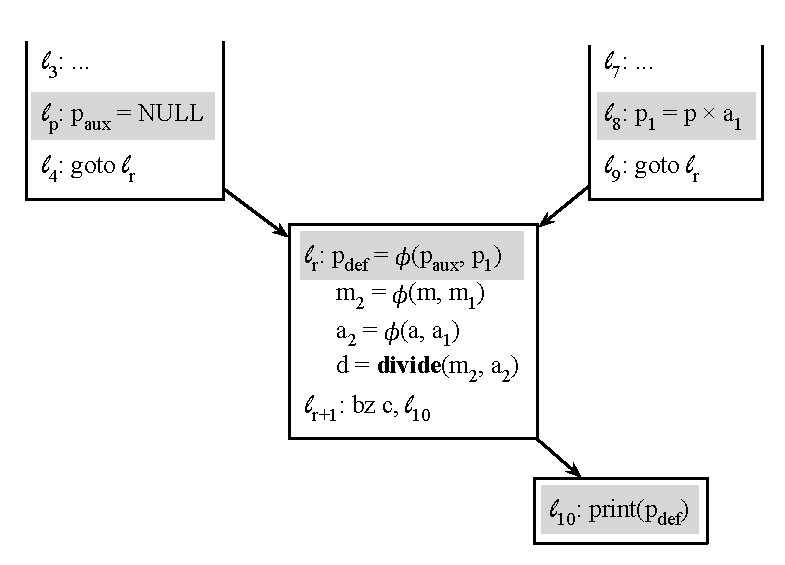
\includegraphics[width=1\columnwidth]{images/Strictify}
\end{center}
\caption{\label{fig:Strictify}
New definitions of $p_1$ to ensure strictness.}
\end{figure}

% Termination
\noindent
\textbf{Termination: }
The function \textbf{merge\_call\_site} always terminates due to a simple
argument: the fusion of two function call sites do not enable the fusion of
further calls.
In other words, if a program has a number $N$ of branches that pass the profit
test performed by the function \textbf{find\_joinable\_calls}; then no more than
$N$ branches will be fused by our optimization.
Therefore, as the number of branches in a program is limited, our algorithm
is guaranteed to terminate.

% Complexity analysis
\noindent
\textbf{Complexity: }
We call function \textbf{merge\_call\_site} recursively at most once per
potentially profitable branch in the program.
Each call of this function scans all the conditional tests in a program,
looking for the most profitable fusion (see line 14 of
\textbf{find\_joinable\_calls} in Figure~\ref{fig:Algorithm0}).
If we have $O(N)$ blocks in the program, we may have to inspect $O(N)$ branches.
Each inspection is $O(N)$, as it involves a traversal of the paths that
sprout away from the conditional.
If two calls must be merged, then we resort to function \textbf{merge\_cfg},
whose complexity is bound by \textbf{strictify\_program}.
This last function is standard in compilers, and runs in $O(N)$.
Therefore, our functions (\textbf{merge\_call\_site}, \textbf{merge\_cfg} and
\textbf{strictify\_program}) run -- together -- in $O(N^4)$.

This complexity may seem very high at a first glance.
However, in practice only a handful of branches lead to two different
calls of the same function.
Furthermore, if we order the branches by profit, then we can inspect each one of
them in line 14 of \textbf{find\_joinable\_calls} at most once.
Therefore, in practice our optimization runs in $O(N^2)$, where $N$ is the 
number of basic blocks in the program code.

\begin{figure}[htb]
\begin{center}
\begin{small}
\begin{tabular}{|c|l|c|c|c|c|} \hline
Cycle   & Instruction                  & $t_0$        & $t_1$        & $t_2$        & $t_3$        \\ \hline
14      & $ c = \tid \% 2$             & $\checkmark$ & $\checkmark$ & $\checkmark$ & $\checkmark$ \\ \hline
15      & $ \code{bz} \ c, then$ & $\checkmark$ & $\checkmark$ & $\checkmark$ & $\checkmark$ \\ \hline
\multicolumn{6}{c}{$\ldots$} \\ \hline
16      & $ m = \tid \ \times \ 1000$        & $\checkmark$    & $\bullet$ & $\checkmark$ & $\bullet$ \\ \hline
17      & $ a = \tid \ + \ 1$ & $\checkmark$    & $\bullet$ & $\checkmark$ & $\bullet$ \\ \hline
\multicolumn{6}{c}{$\ldots$} \\ \hline
25      & $ m1 = \tid \ \times 2000$ & $\bullet$    & $\checkmark$ & $\bullet$ & $\checkmark$ \\ \hline
26      & $ a1 = \tid \ + \ 2$        & $\bullet$    & $\checkmark$    & $\bullet$ & $\checkmark$ \\ \hline
27      & $ p = read()$ & $\bullet$    & $\checkmark$    & $\bullet$ & $\checkmark$ \\ \hline
28      & $ p1 = p \ \times \ a1$ & $\bullet$    & $\checkmark$    & $\bullet$ & $\checkmark$ \\ \hline
\multicolumn{6}{c}{$\ldots$} \\ \hline
45      & $ \code{sync}$        & $\checkmark$ & $\checkmark$ & $\checkmark$ & $\checkmark$ \\ \hline
46      & $ P = phi(m, m1)$    & $\checkmark$ & $\checkmark$ & $\checkmark$ & $\checkmark$ \\ \hline
47      & $ P2 = phi(P, P1)$ & $\checkmark$    & $\checkmark$ & $\checkmark$ & $\checkmark$ \\ \hline
48      & $ d1 = divide(P, P1)$ & $\checkmark$    & $\checkmark$ & $\checkmark$ & $\checkmark$ \\ \hline
\multicolumn{6}{c}{$\ldots$} \\ \hline
49      & $ print(P2)$ & $\bullet$    & $\checkmark$ & $\bullet$ & $\checkmark$ \\ \hline
\multicolumn{6}{c}{$\ldots$} \\ \hline
51      & $ \code{sync}$        & $\checkmark$ & $\checkmark$ & $\checkmark$ & $\checkmark$ \\ \hline
52      & $ print(d1)$ & $\checkmark$    & $\checkmark$ & $\checkmark$ & $\checkmark$ \\ \hline
\end{tabular}

\end{small}
\end{center}
\caption{(Top) The same program from Figure~\ref{fig:exampleOrig} after being optimized.
(Bottom) An execution trace of the program.
If a thread $t$ executes an instruction at cycle
$j$, we mark the entry $(t, j)$ with the symbol $\checkmark$.
Otherwise, we mark it with $\bullet$.}
\label{fig:exampleOpt}
\end{figure}


\section{Experimental Results}
\label{sec:exp}

\paragraph{Experimental setup.}
The fusion of call sites may be applied onto SPMD programs running on SIMD
machines, following the SIMT execution model.
There are several different computer architectures that fit into this model,
from GPUs and vector units (SSE, MMX, etc) to Long's Minimal Multi-Threading
architectures~\cite{Long10}.
As the transformation is performed at source code level, our technique makes no
assumption about the way the SPMD code is later transformed into SIMD
instructions.
Evaluating FCS separately on each programming environment and each platform
would be tedious.
Furthermore, this approach would produce results that are hard to generalise.
Therefore, we chose to evaluate FCS on general-purpose parallel
applications in a micro-architecture-agnostic simulator which models an ideal
SIMT machine.
This simulator has been implemented by Milanez {\em et al.}~\cite{Milanez14},
who have made it publicly available.
The simulator is implemented on top of the PIN binary instrumentation
framework\footnote{\url{http://www.pintool.org/}}.
The Pin tool reads the binary and produces traces representing every
instruction that each thread executes.
Then, we replay the traces using different heuristics (that we describe in the
next paragraph) to re-converge threads.
To perform the code transformation, we have used the LLVM
compiler~\cite{Lattner04}.
Our performance numbers have been obtained in the following way:
we run the PIN-based simulator on the original program that LLVM produces at
its -O3 optimization level.
Then, we apply FCS on that binary, and re-run the simulator.

\noindent
\textbf{Heuristics for Thread Reconvergence:}
our simulator accepts different thread reconvergence heuristics.
Such heuristics determine the next instruction to be fetched in an SIMT
architecture.
We chose to simulate four heuristics: MinPC, MinSP-PC, MaxFun-MinPC, and
Long-MinSP-PC.
These heuristics are described below:
\begin{small}
\begin{description}
\item [Min-PC:] this technique, due to Quinn {\em et al.}~\cite{Quinn88}, is the
thread reconvergence heuristics typically adopted
in the implementation of graphics processing units: in face of divergent
lines of execution, the fetcher always chooses the heuristics with the smallest
Program Counter (PC) to process.
The rational behind this heuristics is simple: in the absence of backward
branches, given two program counters: $n$ and $n+1$, the latter will be executed
after the former.
By fetching the instruction at the lowest PC, the hardware maximizes the chance
of keeping the threads in lockstep execution.

\item [MinSP-PC:] this approach was proposed by Collange~\cite{Collange11} and is 
built on top of Quinn's Min-PC heuristic~\cite{Quinn88}.
It is used in programs that contain function invocations, and its bedrock is 
the fact that when a function is called, the stack grows down.
Thus, threads running more deeply nested function calls have smaller Stack
Pointers (SP).
Based on this observation, this heuristic fetches instructions to threads with the
smallest SP, because it assumes that these threads are behind in the program's 
execution flow.

\item [MaxFun-MinPC:] this heuristic, Maximum Function Level - Minimum PC,
is similar to MinSP-PC, but instead of choosing the smallest SP, it chooses the
thread that has the highest number of activation records on the stack.
Therefore, this heuristic would have the same behavior of MinSP-MinPC if all
activation records had the same size. 

\item [Long:] Long {\em et al.}~\cite{Long10} have created a heuristic to analyze
redundancies in SIMD programs.
Their key idea is to add memory to each thread.
One thread uses the memory of the others to advance or stall.
If the current PC of a thread $t_{0}$ is in the recent history of another
thread $t_{1}$, then thread $t_{0}$ is probably behind $t_{1}$.
In this case, $t_{0}$ needs to progress to catch up with $t_{1}$.
The idea of Long’s heuristic can be used to create other heuristics.
When multiple threads have the same highest priority, the original heuristic
executes these threads alternately, but the variations of Long's heuristic use
other policies to choose the next thread to execute.
In this paper we used Long's with Min-PC: when multiple threads have the
highest priority, the basic block of the threads with smallest PC is executed
first.
Then, all priorities are recounted again for the next choice.
\end{description}
\end{small}

\noindent
\textbf{The Benchmarks:}
To probe the effectiveness of the FCS optimization,
we chose to apply it on general purpose SPMD applications from the PARSEC/SPLASH
benchmark suite~\cite{Bienia08}.
We have used three programs from these collections: \texttt{FFT},
\texttt{Fluidanimate} and \texttt{Swaptions}.
Figure~\ref{fig:benchmarks} shows some characteristics of these benchmarks.
These are the PARSEC programs that we manage to compile using LLVM 3.4.
These programs are large, and contain only a handful of branches that
touch the same function call through different program paths.
Therefore, the benefits that we can expect from the application of FCS on these
benchmarks is limited.
Hence, to demonstrate the possibilities of our optimization, we shall apply it
also onto the program first seen in Figure~\ref{fig:exampleOrig}.

\begin{figure}[t!]
\begin{small}
\renewcommand\arraystretch{1.2}
\begin{center}
\begin{tabular}{l|rrrr}
\textbf{Benchmark} & \textbf{LoC} & \textbf{Inst} & \textbf{Trace} &
\textbf{Merge} \\ \hline
Divide       &    51 &   112 &   581 & 1 \\
FFT          & 1,291 & 2,854 &   697 & 4 \\
Fluidanimate & 5,712 & 6,357 & 5,586 & 3 \\
Swaptions    & 1,309 & 3,742 & 1,123 & 3
\end{tabular}
\end{center}
\caption{The benchmarks that we have analyzed.
\textbf{LoC}: number of lines of code, including comments;
\textbf{Inst}: number of assembly instructions;
\textbf{Trace}: number of instructions in millions, that each benchmark
executes with its standard input
\textbf{Merge}: number of call sites that we have merged.}
\label{fig:benchmarks}
\end{small}
\end{figure}

% Divide: 1
% FFT: 4
% Fluidanimate: 3
% Swaptions: 3

\noindent
\textbf{Performance analysis:}
Figure~\ref{fig:Results} shows the result of combining our optimization with
different heuristics and different numbers of available threads.
Numbers above bars show relative speedup compared to not using our optimization.
We performed these experiments on an Intel Xeon CPU E5-2620 2.00GHz processor
with 16 GB of DDR2 RAM running Linux running Ubuntu 12.04 (Kernel 3.2.0).
Nevertheless, our results do not dependend on these features, as they
have been produced through simulation.
Our experiments let us draw some conclusions.
MinPC-based heuristics (MinSP-PC and MinPC) tend to benefit more from FCS.
This advantage exists because such heuristics favour the synchonization of threads
before a function call.
For instance, in Figure~\ref{fig:Algorithm1} both, MinPC and MinSP-PC, will
fetch the instructions in all the smaller labels, e.g., $\ell_2 - \ell_9$, before
grabbing $\ell_r$, which lays further ahead in the program's binary layout.
Consequently, the heuristic published by Long {\em et al.} does not benefit as
much, because it has been designed in a way that is totally oblivious to the
invocation of functions.
Figure~\ref{fig:Results} also shows that our optimization does not impact
negatively the benchmarks that we have tested.
The only exceptions are due to MinPC in Swaptions (four threads) and in
FFt (16 threads).
This negative impact is due to back-edges, e.g., jumps that lead the
program's flow back to the beginning of a loop.
In face of repeat-style iterators, which test the exit condition at the end,
MinPC may fail to reconverge threads within the loop.
In this case, the slightly larger code that we produce ends up causing an
increase on the number of instructions that are not shared among threads.
We have not observed this behavior in the other heuristics.

\begin{figure}[t!]
\begin{center}
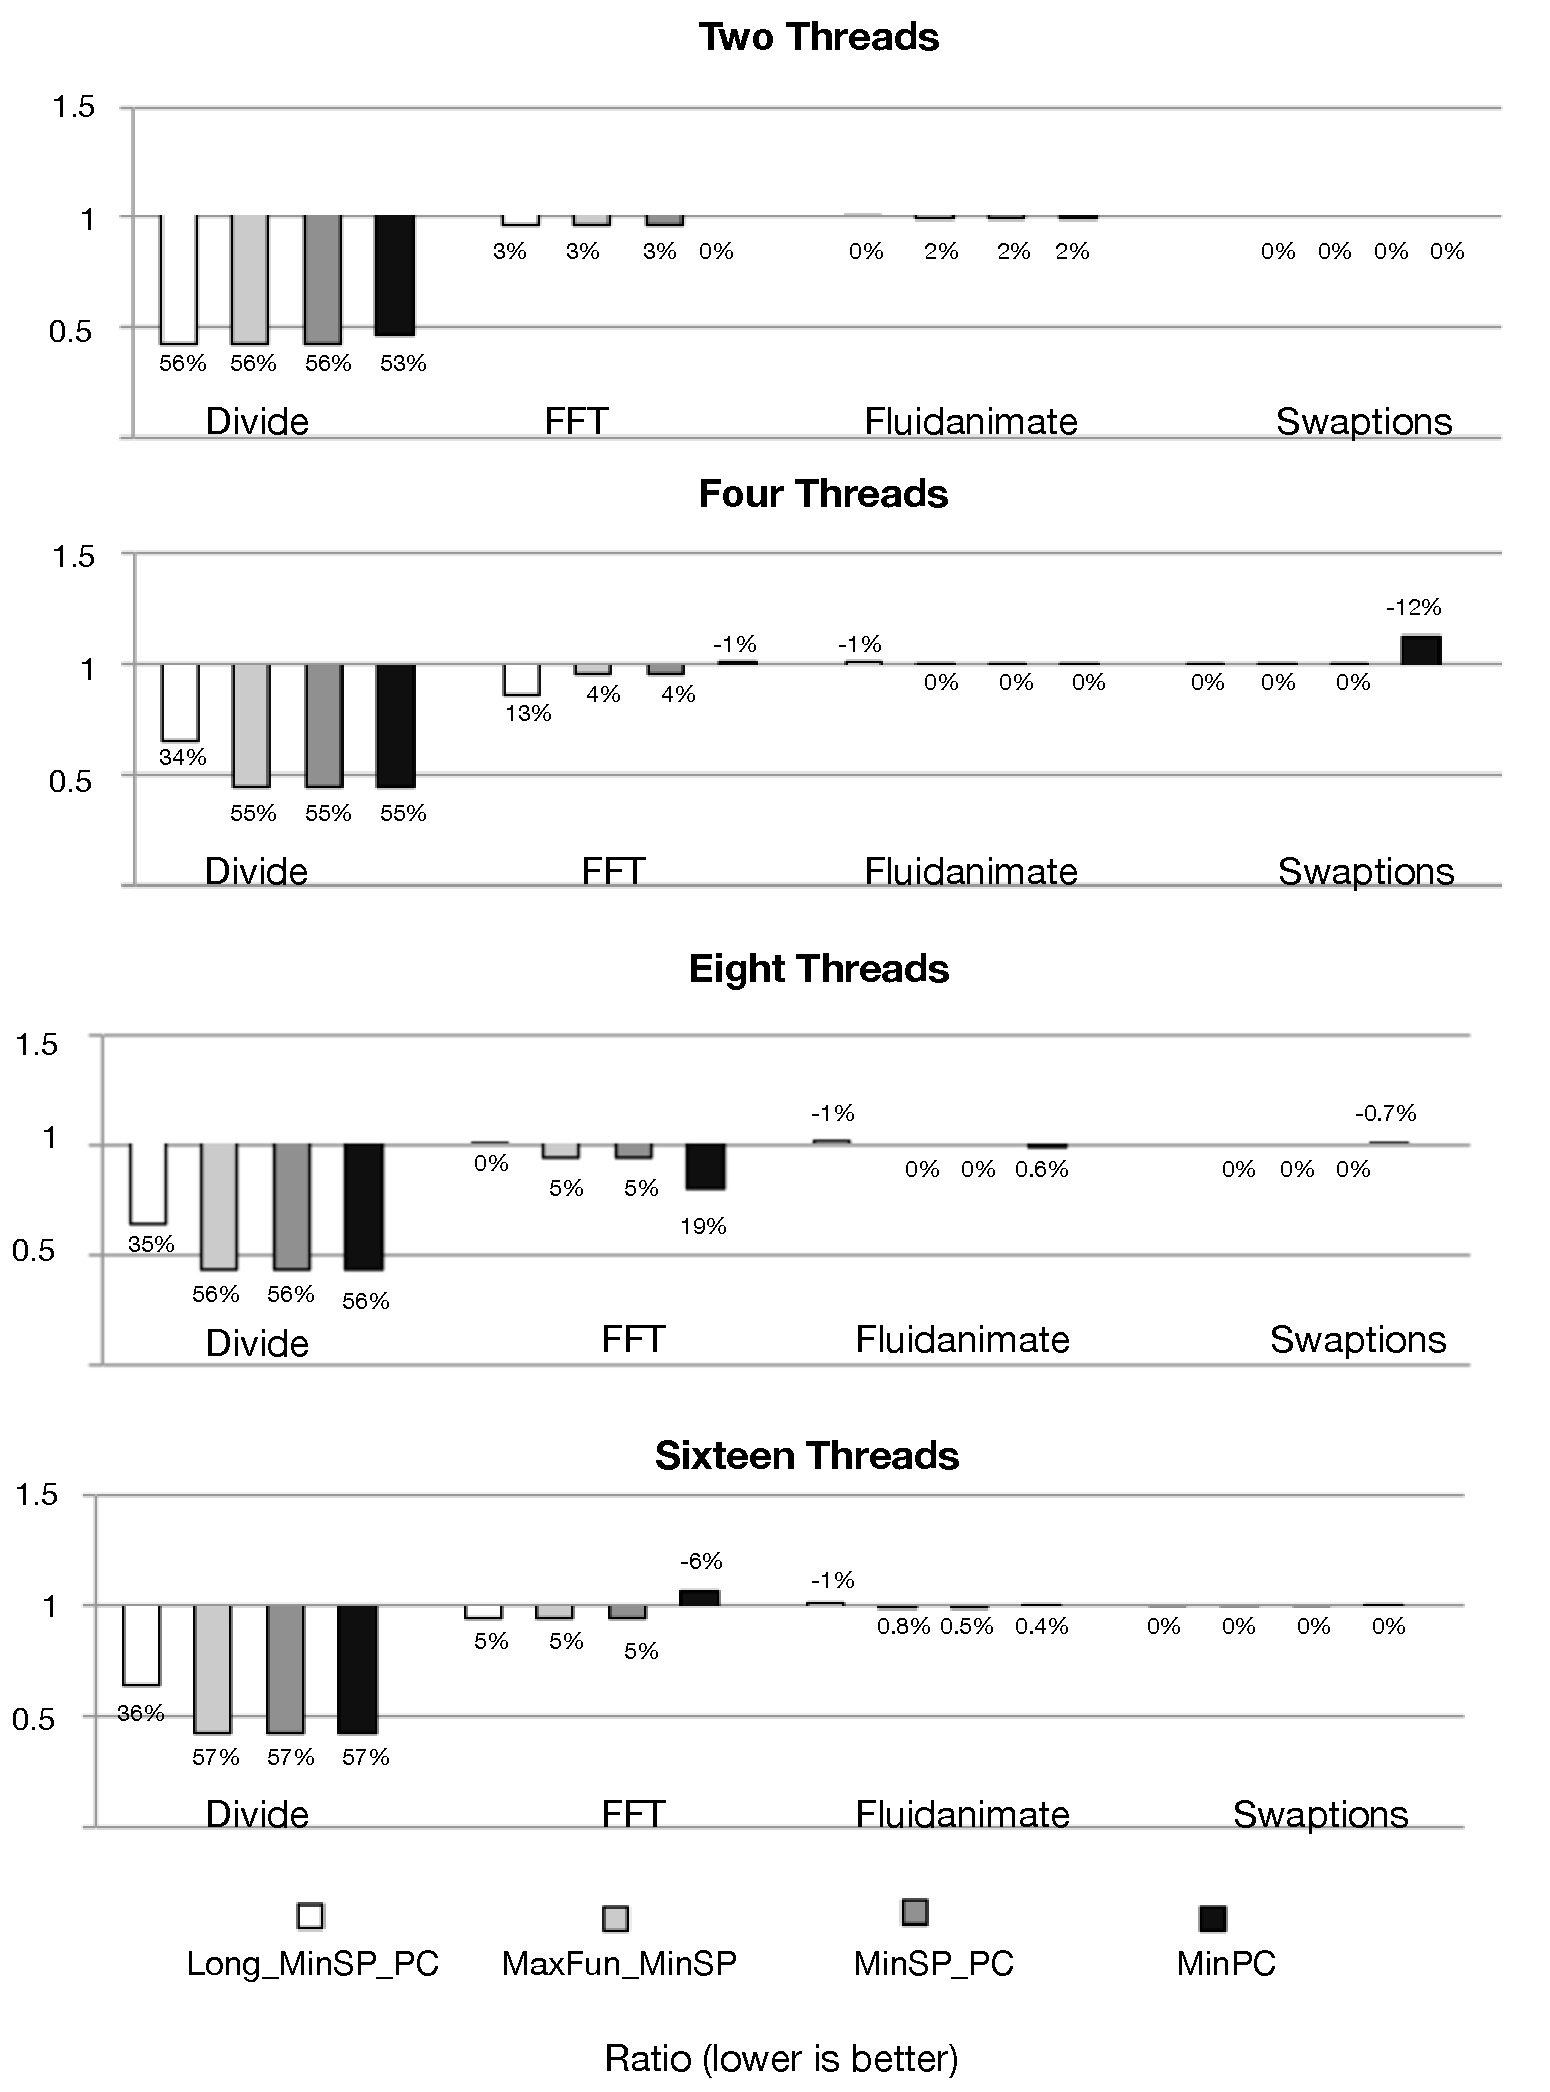
\includegraphics[width=1\columnwidth]{images/ResultsFuncFusion}
\end{center}
\caption{\label{fig:Results}
Execution time reduction after applying FCS.}
\end{figure}


\section{Related Work}
\label{sec:rw}

\noindent
\textbf{Other Divergence Aware Optimizations:} this paper introduces a new
optimization to mitigate the performance loss
caused by divergences in GPGPU applications.
There are a number of different optimizations that serve the same purpose;
however, they reduce divergences in different
ways~\cite{Carrillo09,Coutinho11,Han11,Lee09,Zhang10a,Zhang11}.
For instance, Han {\em et al.}'s~\cite{Han11} {\em Branch Distribution}
hoists instructions up or down divergence paths to join them at common
program points -- we can perform this merging in the middle of divergence paths.
{\em Branch Fusion}~\cite{Coutinho11} is a generalization of Branch Distribution;
however, it does not merge function calls.
In other words, the optimization of Coutinho {\em et al.} bails out when faced
with divergent branches that contain call instructions -- this is the exact
case that we handle.

There are other divergence aware optimizations that target loops, instead of
branches, as we do.
For instance, Carrillo {\em et al.}~\cite{Carrillo09} have designed a code
transformation called {\em Branch Splitting}, which divides parallelizable loops
enclosing multi-path branches.
In this way, they produce multiple loops, each one with a single control flow
path.
In similar lines, Lee {\em et al.}~\cite{Lee09} have proposed {\em Loop
Collapsing}, a technique that reduces divergences by combining multiple
divergence loops into common iterators.
Han {\em et al.}~\cite{Han11} have further extended Lee's approach with the
notion of {\em Iteration Delaying}.
This transformation recombines loops containing divergent branches, so that
threads tend to remain together for a longer time.
None of these optimizations is designed to handle
function calls specifically, and, more importantly: none of them would be
able to carry out the optimization that we discuss in this paper.

\noindent
\textbf{Function-Aware Heuristics to Reconverge Threads:}
there exist different heuristics implemented at the hardware level that
enforce early reconvergence of divergent
threads~\cite{Dechene10,Gonzalez08,Long10}.
In particular, Milanez {\em et al.}~\cite{Milanez14} have proposed the
Min-SP-PC technique, one of the heuristics that we use in this paper.
We emphasize that our work is orthogonal and complementary to these research
efforts.
Our optimization can be applied on programs independent on the heuristic
used to reconverge threads.
Nevertheless, as we have observed in Section~\ref{sec:exp}, some of these
heuristics yield greater benefit when combined with our approach.

\section{Conclusion}
\label{sec:con}

This paper has introduced Fusion of calling sites, a new compiler optimization that mitigates the
negative impact caused by divergences on applications running in SIMD fashion.
This optimization consists in rearranging the control flow graph of a program,
so to merge different function call sites at common program points.
In this way, the merged function can be invoked together by divergent
threads.
There exists, presently, a great deal of effort to develop techniques, at the
hardware and software level, to reduce the effects of divergences.
Our work is complementary to these efforts: our gains are cumulative with
the increasing performance of graphics cards, and it adds a negligible cost
over compilation time.
More importantly, we believe that optimizations such as Fusion of calling sites
contribute to shield application developers from particularities of
the parallel hardware, such as divergence and reconvergence of threads.

\noindent
\textbf{Software: } the software used in this paper, including our simulator
and binary instrumentation tool, is available at \url{https://github.com/dougct/function-call-fusion}.


\bibliographystyle{IEEEtran}
\bibliography{references}

\end{document}
